\chapter{Estimador analógico} \chapterlabel{Informe/5-EstimadorAnalogico} \label{cap:Estimador Analogico}

Para que la placa de control pueda mantener la distancia de separación de entrehierro $Y_{g}$ es necesario conocer su valor para luego actuar en consecuencia. Si bien se podrían utilizar sensores  especializados para ello, para este proyecto se optó por medirla de manera indirecta a partir de la pendiente de la corriente que circula por el electroimán. De esta forma, se logran aplicar conceptos de estimación de variables, aprendidos durante la carrera. 

En este capítulo se detalla la estrategia utilizada para realizar la estimación de posición a partir de la corriente del electroimán, junto con el diseño circuital y sus respectivas simulaciones. Finalmente se obtiene una función transferencia del bloque estimador que será luego utilizada para el diseño del compensador analógico.

\section{Análisis de la estimación}\label{analisis_de_estimacion}

Como se analizó en el capítulo \ref{cap:ControladorCorriente}, para controlar el valor medio de la corriente se utiliza una fuente conmutada que alterna la polaridad de la tensión aplicada al electroimán. Esto genera una onda de corriente triangular superpuesta al valor medio deseado, cuyas pendientes de crecimiento y de decrecimiento contienen información de la distancia de separación de entrehierro. Por lo tanto, se decidió realizar una estimación de la distancia a partir de la medición de dichas pendientes.

En la sección \ref{sec_analisis_estimacion} se obtuvo una ecuación que relaciona la pendiente de la corriente con la inductancia del electroimán. De esta forma, al reemplazar en la ecuación \ref{eq_derivada_corriente_2} dicha inductancia por su expresión linealizada \ref{eq_induct_practica}, obtenida a partir de mediciones, se obtiene:

\begin{equation} \label{eq_derivada_corriente_3}
	\frac{di_L(t)}{dt}= \frac{V_L}{L(Y_g)}=\frac{V_L}{-2.56*Y_{g}+0.027}
\end{equation}

Debido a que la alimentación $V_L$ del electroimán tiene dos valores posibles $V_L=+V_{cc}$ o $V_L=-V{cc}$, se puede reescribir la expresión \ref{eq_derivada_corriente_3} en función de $V_{cc}$:
\colorbox{red}{Y si ponemos directamente 24V?}

\begin{equation} \label{eq_derivada_corriente_4}
	\left|\frac{di_L(t)}{dt}\right|= \frac{V_{cc}}{L(Y_g)}=\frac{V_{cc}}{-2.56*Y_{g}+0.027}
\end{equation}

A partir de la expresión \ref{eq_derivada_corriente_4} se evalúa la derivada para distintos valores de distancia y se obtiene la tabla \ref{tab_derivada_linealizada}.

\begin{table}[H]
	\begin{center}
		\begin{tabular}{| c | c |}
			\hline
			$Y_g[\:mm]$ & $\abs{\frac{di_L(t)}{dt}} [\:\frac{A}{s}]$\\ \hline
			2 & 1091.9 \\ \hline 
			3 & 1235.8 \\ \hline 
			4 & 1423.5 \\ \hline 
			5 & 1678.3 \\ \hline 
		\end{tabular}
		\caption{Pendiente de la corriente en función de la distancia de entrehierro.}
		\label{tab_derivada_linealizada}
	\end{center}
\end{table}

Se realiza una regresión por mínimos cuadrados a los valores de la tabla \ref{tab_derivada_linealizada} y se obtiene una expresión linealizada de la pendiente, que se  muestra en la ecuación \ref{eq_di-dt_lineal}.


\begin{equation} \label{eq_di-dt_lineal}
	{\left|\frac{di_L}{dt}\right|}_{Lineal}[\:\frac{A}{s}]= 194690 * Y_g\:[m]+676
\end{equation}

Al despejar la distancia de separación se obtiene:

\begin{equation} \label{eq_Yg_despejada}
	Y_g\:[m] =5.136*10^{-6}*{\left|\frac{di_L}{dt}\right|}_{Lineal} - 3.472*10^{-3}
\end{equation}


En la expresión \ref{eq_Yg_despejada} se puede observar que, para obtener una estimación de la distancia de separación, es necesario medir el módulo de la pendiente de la onda triangular de la corriente en el electroimán. Para realizar la estimación a partir de un circuito analógico se propone implementar un circuito derivador que permita obtener la pendiente de la corriente. Como esta tiene forma triangular, estará compuesta por un segmento creciente (pendiente positiva) y uno decreciente (pendiente negativa). Debido a que en la expresión \ref{eq_Yg_despejada} se necesita obtener su módulo, se agrega una etapa de rectificación a la salida del derivador.

La forma de onda correspondiente a la salida de cada etapa a implementar se muestra en la figura \ref{fig:img_forma-de-onda-estimador}. En ella se observa que se parte con una onda triangular, correspondiente a la corriente que circula por el electroimán. Luego, al pasar por el derivador, se obtiene una onda pulsada, cuyos valor superior e inferior se corresponden con la pendiente de crecimiento y de decrecimiento de la corriente. Luego, al entrar a la etapa de rectificación se obtiene un valor constante y proporcional a la pendiente y, por ende, a la distancia de separación de entrehierro.


\begin{figure}[H]
	\centering
	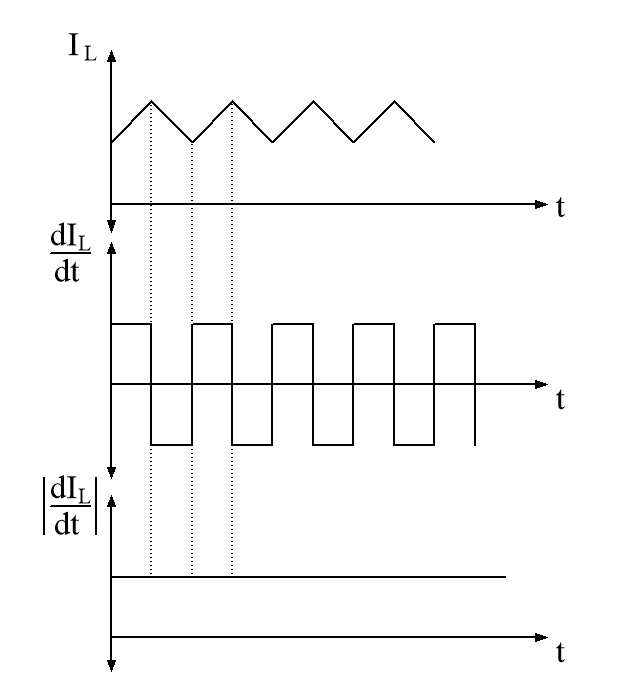
\includegraphics[scale=0.7]{forma-de-onda-estimador.png}
	\caption{Formas de onda de cada etapa del estimador.}
	\label{fig:img_forma-de-onda-estimador}
\end{figure}



Hasta ahora se planteó que la entrada al derivador es la corriente del electroimán. Sin embargo, esta no es medida de manera directa, sino que se mide a través del sensor de efecto Hall, cuya salida es $V_{IL_{feed}}$ (\ref{eq_salida_restador_hall_2}). Por lo tanto es necesario tener en cuenta su ganancia $H_0$ al momento de diseñar el estimador. La expresión a implementar circuitalmente resulta:

\begin{equation} \label{eq_Yg_salida_sensor}
	Y_g=\frac{5.136*10^{-6}}{H_0}*{\left|\frac{dV_{IL_{feed}}}{dt}\right|}_{Lineal} - 3.472*10^{-3}
\end{equation}

%Además se decidió agregar un LPF luego del rectificador para reducir las frecuencias no deseadas introducidas por el cambio de signo de la pendiente, las cuales generan saltos sobre un punto de operación en la tensión de salida del derivador.
El diagrama en bloques que describe cómo está conformado el estimador se muestra en la figura \ref{fig:img_diag-en-bloques_estimador}. En ella se observa que la señal de entrada es la tensión de salida del sensor de efecto Hall, que ingresa al circuito derivador obteniéndose $V_{deriv}$. Finalmente, esta señal es rectificada y se obtiene $V_{estim}$, que es proporcional a la distancia de separación de entrehierro.

\begin{figure}[H]
	\centering
	%Acá se define eñ diagrama en bloques completo
\begin{tikzpicture}[auto, node distance=2.5cm,>=latex']
	% We start by placing the blocks
	\node [input, name=input] {};
	\node [block, right of=input] (derivador) {$DERIVADOR$};

	\node [block, right of=derivador, 
	node distance=4.5cm] (modulo) {$|.|$};
	\node [output, right of=modulo] (output) {};

	% Once the nodes are placed, connecting them is easy. 
	\draw [draw,->] (input) -- node[pos=0.1]{$V_{IL_{feed}}$} (derivador);
	\draw [draw,->] (derivador) -- node{$V_{deriv}$} (modulo);
	\draw [->] (modulo) -- node [name=y] {$V_{estim}$}(output);
\end{tikzpicture}


	
	\caption{Diagrama en bloques simplificado del estimador.}	\label{fig:img_diag-en-bloques_estimador}
\end{figure}

A continuación se diseña la implementación circuital de cada una de las etapas que componen al diagrama en bloques \ref{fig:img_diag-en-bloques_estimador}.

{
	%Por lo tanto, en esta capítulo/sección.. se aborda el análisis de la implementación…
	
	%En el capítulo 3 se analizó la forma de onda resultante de la corriente del electroimán al ser excitado con una fuente conmutada. Esta resulta en una onda triangular con un valor medio deseado, cuya pendiente de crecimiento y de decrecimiento varía proporcionalmente con distancia de separación de entrehierro. A partir de esto, se decidió realizar una estimación de la misma a partir de la medición de la pendiente de la onda triangular de la corriente.
}


\section{Diseño circuital del estimador de posición}
\colorbox{red}{Breve resumen?}

\subsection{Circuito derivador}

Para poder obtener $\frac{dV_{IL_{feed}}}{dt}$ se utiliza un circuito derivador basado en un amplificador operacional como el que se muestra en la figura \ref{fig:img_Circuito-derivador}. Se decide utilizar amplificadores operacionales alimentados con una fuente de tensión simple de $5\:V$ con una excursión completa en su salida. 

Debido a que $V_{IL_{feed}}$ es una onda triangular, su derivada será una onda pulsada. Por lo tanto, para poder representar valores de pendientes tanto positivos como negativos es necesario polarizar la salida del derivador en un punto de operación ($V_{op}$) para no perder información. Como la salida varía entre $0\:V$ y $5\:V$ se utiliza $V_{op}=2.5\:V$ para permitir igual excursión en ambos sentidos.

\begin{figure}[H]
	\centering
	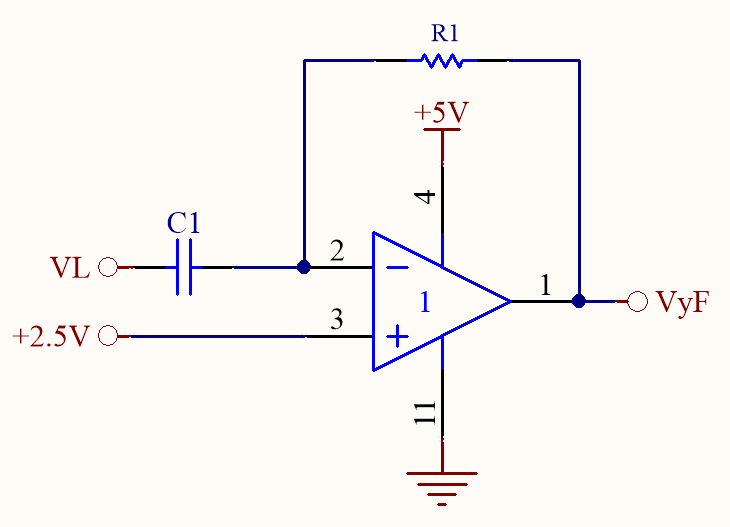
\includegraphics[scale=0.5]{Circuito-derivador.png}
	\caption{Circuito derivador.}
	\label{fig:img_Circuito-derivador}
\end{figure}


La salida del circuito $V_{deriv}(t)$ ante su entrada $V_{IL_{feed}}$ es:

\begin{equation} 
	V_{deriv}(t)\ = V_{op} - \frac{dV_{IL_{feed}}}{dt}*C_1*R_1
\end{equation}

Teniendo en cuenta que $V_{IL_{feed}}=I_L*H_0+0.1\:V$, al hacer su derivada se pierde el término constante, entonces $ \frac{dV_{IL_{feed}}}{dt}= \frac{dI_L}{dt}*H_0$. Por lo tanto, se obtiene:

\begin{equation} \label{eq_vyf1}
	V_{deriv}(t) = 2.5\:V\ -\frac{dI_L}{dt}*H_0*C_1*R_1
\end{equation}

Según la expresión \ref{eq_vyf1}, la salida del derivador $V_{deriv}$ excursionará alrededor de $V_{op}=2.5\:V$ con un valor máximo de $5\:V$ y un mínimo de $0\:V$. Cualquier valor que supere esos límites provocaría una saturación del amplificador operacional.

Para evitar una saturación de la salida del derivador y teniendo en cuenta que $V_{deriv}(t)$ presenta variaciones alrededor del punto de operación de $2.5\:V$ se debe cumplir, para todos los casos posibles de pendiente en el rango de distancia de trabajo, que:

\begin{equation} \label{eq_vyf3}
	\left|-\frac{dI_L}{dt}*H_0*C_1*R_1\right|\ \le 2.5\:V
\end{equation}

Por lo tanto, con la ecuación \ref{eq_derivada_corriente_2} y \ref{eq_vyf3} se plantea que:

\begin{equation} \label{eq_condicionC1-R1}
	C_1*R_1\le\frac{2.5\ \:V\ *L_{min}}{V_{cc}*H_0}
\end{equation}

Con $L_{min}= L(5\: mm) = 14.9\: mHy$ se obtiene: 

\begin{equation} \label{eq_condicionC1-R1-2}
	C_1*R_1\le\ 29.1\ ms
\end{equation}

El derivador tiene como salida una onda pulsada, cuyo nivel superior es proporcional a la pendiente de bajada de la corriente en el electroimán, y el nivel inferior es proporcional a la pendiente de subida.

Para los cálculos se utilizó $\tau = C_1*R_1= 25\:ms$, para dar un margen y evitar la saturación del amplificador operacional.  

Con la ecuación \ref{eq_di-dt_lineal} y \ref{eq_vyf1}, y con una variación en torno a $2.5\:V$ se obtienen dos expresiónes para la salida del derivador en función de la distancia de entrehierro y el sentido de las pendientes.


%\begin{equation} \label{eq_Vyf-lineal}
%	V_{deriv}(Y_g)\:[V] =\ |H_0*C_1*R_1*\frac{di_L}{dt}| +2.5=0.2595*Y_g[mm]+3.4
%\end{equation}

Para pendiente positiva, la salida del circuito derivador resulta:

\begin{equation} \label{eq_Vyf-lineal-pos}
	V_{deriv}(Y_g) = -0.2595*Y_g[mm] + 1.6\:V
\end{equation}


Para pendiente negativa:

\begin{equation} \label{eq_Vyf-lineal-neg}
	V_{deriv}(Y_g) = 0.2595*Y_g[mm] + 3.4\:V
\end{equation}


A partir de la expresiones \ref{eq_Vyf-lineal-pos} y \ref{eq_Vyf-lineal-neg} se realizó la tabla \ref{tab_Vyf_vs_y} que muestra el valor de salida del derivador para distintos valores de distancia de entrehierro. Se puede observar que la tensión de salida del derivador se mantiene entre $0\:V$ y $5\:V$.

\begin{table}[H]
	\begin{center}
		\begin{tabular}{| c | c | c |}
			\hline
			$Y_g[\:mm]$ & $V_{deriv_{sup}}(Y_g) [\:V]$ & $V_{deriv_{inf}}(Y_g) [\:V]$
			\\ \hline
			2 & 3.92 & 1.08\\ \hline 
			3 & 4.18 & 0.82\\ \hline 
			4 & 4.44 & 0.56\\ \hline 
			5 & 4.7  & 0.30\\ \hline 
		\end{tabular}
		\caption{Tensión de salida del derivador ($V_{deriv}$) en función de la posición ($Y_g$).}
		\label{tab_Vyf_vs_y}
	\end{center}
\end{table}

Al observar los valores superiores e inferiores obtenidos en la tabla \ref{tab_Vyf_vs_y}, se puede ver que para cada valor de $Y_g$, los valores obtenidos tienen una excursión ($\Delta V_{deriv}$) simétrica alrededor de $2.5\:V$. Por lo tanto, se puede expresar la salida del derivador como se muestra en las expresiones \ref{eq_vderiv_pos} y \ref{eq_vderiv_neg}.

Para pendiente positiva:

\begin{equation}\label{eq_vderiv_pos}
	V_{deriv}=2.5\:V - \abs{\Delta V_{deriv}}
\end{equation} 


Para pendiente negativa:

\begin{equation}\label{eq_vderiv_neg}
	V_{deriv}=2.5\:V + \abs{\Delta V_{deriv}}
\end{equation} 



\subsection{Circuito del derivador compensado}

En esta sección se analiza la respuesta en frecuencia del circuito derivador. Para su implementación se propone utilizar el amplificador operacional MCP660, el cual fue  también utilizado en el diseño circuital del controlador de corriente. Este es internamente compensado, por lo que todos sus otros polos los tiene luego del cruce por $0\:dB$ de la ganancia. Para simplificar el análisis estos no se tienen en cuenta, ya que están fuera de la zona de interés. Su ganancia de lazo abierto es:

\begin{equation} \label{eq_Aw_1}
	A(s)=\frac{1778279}{(\frac{s}{2\pi *20}+1)}
\end{equation} 

La estabilidad del circuito derivador puede analizarse a partir del diagrama en bloques que se muestra a continuación:

\begin{figure}[H]
	\centering
	%Acá se define eñ diagrama en bloques completo
\begin{tikzpicture}[auto, node distance=3.5cm,>=latex']
	% We start by placing the blocks
	\node [input, name=input] {};
	\node [block, right of=input] (Gin) {$G_{in}(s)$};
	\node [sum, right of=Gin, node distance=3.5cm] (suma) {+};
	
	\node [block, right of=suma] (amplificador) {$A(s)$};
	\node [output, right of=amplificador] (output) {};
	\node [block, below of=amplificador] (realimentacion) {$H(s)$};
	
	
	% Once the nodes are placed, connecting them is easy. 
	\draw [draw,->] (input) -- node[pos=0.1]{$V_{IL_{feed}}$} (Gin);
	\draw [draw,->] (Gin) -- node[pos=0.9]{-}(suma);
	\draw [draw,->] (suma) -- (amplificador);
	\draw [draw,->] (amplificador) -- node[name=y]{$V_{deriv}$} (output);
	\draw [->] (y) |- (realimentacion);
	\draw [->] (realimentacion) -| node[pos=0.99]{-} (suma);
\end{tikzpicture}
	\caption{Diagrama en bloques del circuito derivador.}	\label{fig:img_diag-en-bloques_derivador}
\end{figure}



La red de realimentación $H(s)$ y la ganancia de entrada $G_{in}(s)$ están dadas por el circuito formado por $C_1$ y $R_1$ en la figura \ref{fig:img_Circuito-derivador}.

\begin{equation}
	G_{in}(s)=\frac{s*C_1*R_1}{1+s*C_1*R_1}
\end{equation}

\begin{equation}
	H(s)=\frac{1}{1+s*C_1*R_1}
\end{equation}

Para el análisis de estabilidad se realiza el diagrama de Bode de la ganancia del amplificador operacional ($A(s)$) junto con la inversa de la ganancia de realimentación, que resulta:

\begin{equation} \label{eq_Aw_2}
	\frac{1}{H(s)}=1+s*C_1*R_1
\end{equation}

En la figura \ref{fig:img_MCP_sin_compensar} se muestra el diagrama de Bode de A(s) y $\frac{1}{H(s)}$. En ella se puede observar que cuando ambas curvas se cruzan ($\abs{G*H}=1$), la contribución en fase de ambas es de 180º, por lo tanto el circuito resulta inestable. 

\begin{figure}[H]
	\centering
	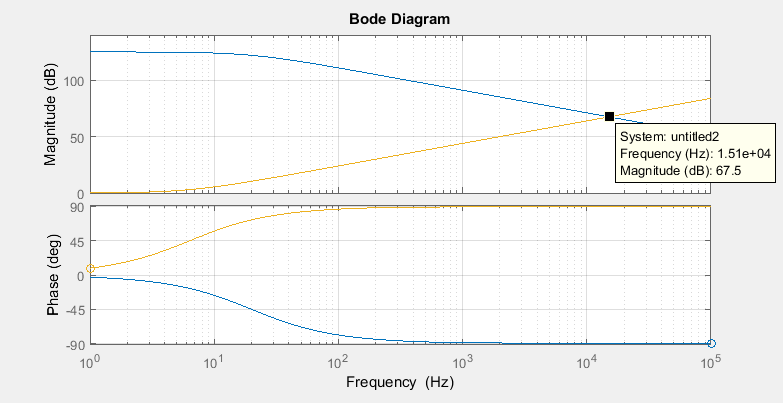
\includegraphics[scale=0.7]{MCP_sin_compensar.png}
	\caption{Respuesta en frecuencia del amplificador operacional MCP660 y de la red de realimentación sin compensar.}
	\label{fig:img_MCP_sin_compensar}
\end{figure}

Debido a la inestabilidad del circuito derivador es necesario compensarlo mediante el agregado de un polo en $\frac{1}{H(s)}$ de forma tal que, cuando ambas curvas se crucen, la suma de fase sea menor a 180º. Esto se logra agregando una resistencia ($R_2$) en serie al capacitor, como se observa en la figura \ref{fig:img_Circuito_derivador_compensado}. De esta forma, la inversa de la red de realimentación resulta:

\begin{equation} \label{eq_MCP_compensado}
	\frac{1}{H(s)}=\frac{1+s*C_1*(R_1+R_2)}{1+s*C_1*R_2}
\end{equation}

\begin{figure}[H]
	\centering
	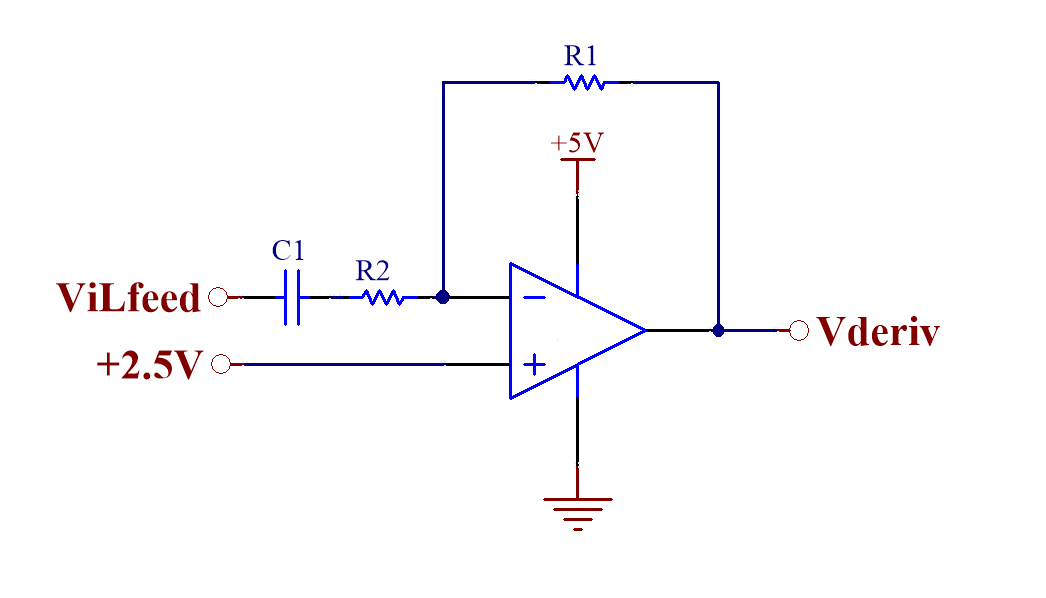
\includegraphics[scale=0.5]{Circuito-derivador- compensado.png}
	\caption{Circuito derivador compensado.}
	\label{fig:img_Circuito_derivador_compensado}
\end{figure}

Al agregar esta compensación el circuito deja de comportarse como derivador a partir de la frecuencia del polo agregado en $\frac{1}{H(s)}$. Por lo tanto, esta frecuencia debe ser mayor a la quinta armónica de la onda triangular de corriente. De la tabla \ref{tab_mediciones} se obtiene que la frecuencia fundamental máxima a la que trabaja el sistema (para $Y_g=5\:mm$) es de $1632.35\:Hz$, por lo que al considerar su quinta armónica se obtiene una frecuencia de $8161\:Hz$. 

Por lo tanto, se ubica el polo de la compensación en $16\:kHz$ para maximizar el ancho de banda del derivador, logrando un margen de fase de aproximadamente 45º. Esto da como resultado $R_2=10\:\Omega$, $C_1=1\:uF$ y $R_1=25\: k\Omega$. El bode de la ganancia a lazo abierto del amplificador operacional junto con su red de realimentación $\frac{1}{H(s)}$ con el cero agregado se observa en la figura \ref{fig:img_MCP_compensado}.

\begin{figure}[H]
	\centering
	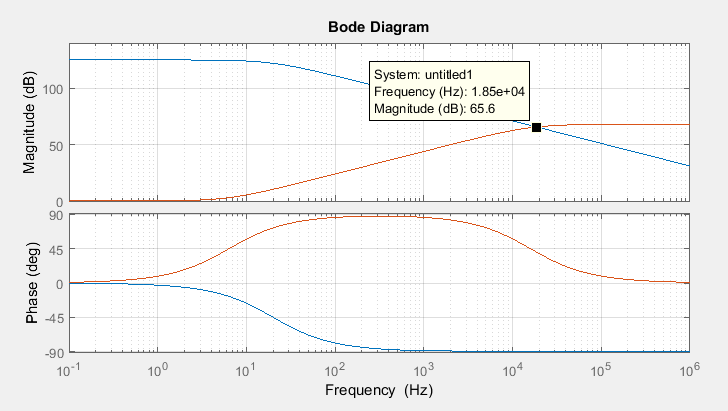
\includegraphics[scale=0.7]{MCP_compensado.png}
	\caption{Respuesta en frecuencia del amplificador operacional MCP660 y de la red de realimentación compensado.}
	\label{fig:img_MCP_compensado}
\end{figure}

En la figura \ref{fig:img_GH del derivador compensado} se muestra la magnitud y la fase de la transferencia a lazo abierto (G(s)*H(s)). En ella se puede observar que el margen de fase resultante es de $\phi =49.6{}^\circ $ y el ancho de banda es de $18.7\:kHz$.

\begin{figure}[H]
	\centering
	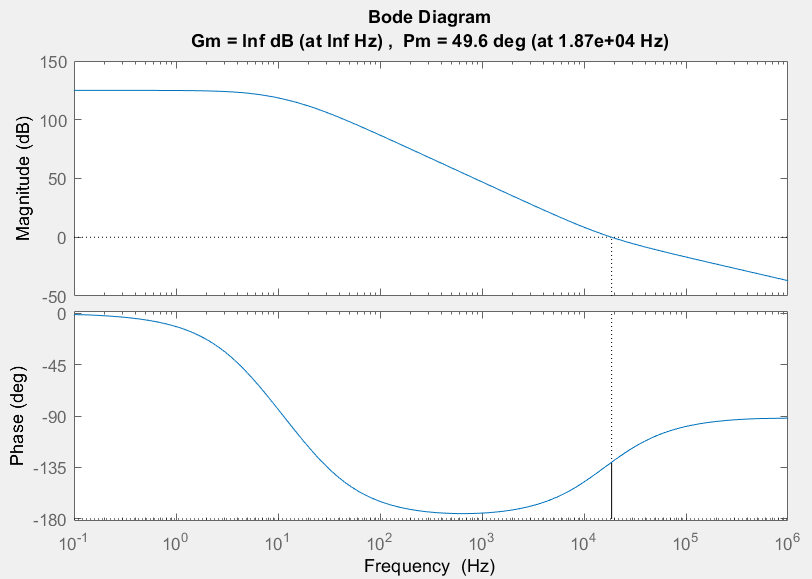
\includegraphics[scale=0.5]{GH-del-derivador-compensado.png}
	\caption{Transferencia a lazo abierto del derivador compensado.}
	\label{fig:img_GH del derivador compensado}
\end{figure}

Finalmente, en la figura \ref{fig:img_Transferencia-de-lazo-cerrado} se muestra la transferencia de lazo cerrado (TLC), que tiene un comportamiento derivativo hasta aproximadamente $18 \:kHz$. 


\begin{figure}[H]
	\centering
	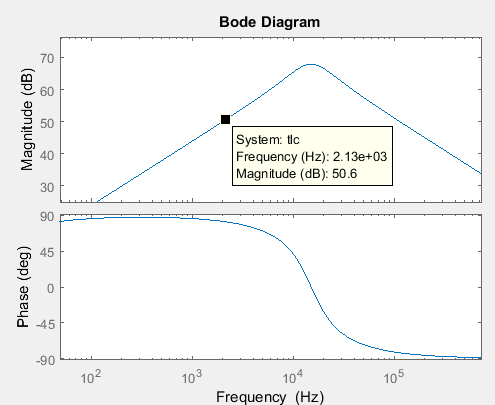
\includegraphics[scale=0.7]{Transferencia-de-lazo-cerrado.png}
	\caption{Transferencia de lazo cerrado.}
	\label{fig:img_Transferencia-de-lazo-cerrado}
\end{figure}


A continuación se muestra la TLC del circuito derivador:

\begin{equation} \label{eq_TLC_derivador}
	{TLC}_{derivador}=\frac{V_{deriv}}{V_{iL_{feed}}}=\frac{-0.025*s}{1+(\frac{2*0.473}{94.5\: k})*s+(\frac{s}{94.5\:k})^2}
\end{equation} 

\section{Etapa de rectificación}

Como se mencionó en la sección \ref{analisis_de_estimacion}, es necesario obtener el valor absoluto de la salida del derivador para tener a la salida del estimador una señal aproximadamente continua. Es por ello que se implementa un circuito rectificador en la salida del derivador alrededor de $V_{op}=2.5\:V$.

Para la implementación circuital del rectificador se decidió utilizar la misma topología usada en la versión anterior del prototipo, que se muestra en la figura \ref{fig:img_Circuito_estimador_de_posición_completo}. Este circuito está compuesto por tres etapas: rectificación, resta y filtrado. Para facilitar su comprensión se realiza un análisis de cada una de estas etapas por separado.

\begin{figure}[H]
	\centering
	\includegraphics[scale=0.6]{Circuito-estimador-de-posición-completo.png}
	\caption{Circuito de rectificación, resta y filtrado.}
	\label{fig:img_Circuito_estimador_de_posición_completo}
\end{figure}

\subsection{Rectificador}

Para entender el funcionamiento del rectificador, se comienza con el análisis de la primer etapa del circuito de la figura \ref{fig:img_Circuito_estimador_de_posición_completo}. Por lo tanto, se simplifica el circuito al mostrado en la figura \ref{fig:img_Rectificador_y_restador}. Se parte de la suposición de que en un amplificador operacional ideal, la tensión diferencial ($V_d$) es igual a cero. De esta forma, como la entrada no inversora está fijada en $2.5\:V$, la misma tensión se encuentra en la entrada inversora.


\begin{figure}[H]
	\centering
	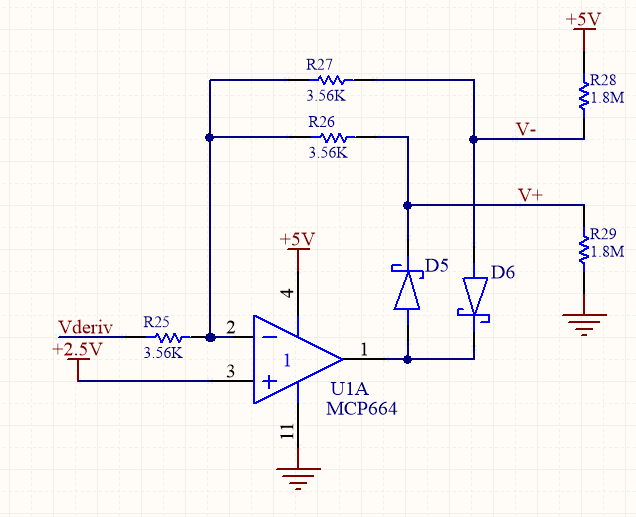
\includegraphics[scale=0.6]{Rectificador-y-restador.png}
	\caption{Circuito rectificador.}
	\label{fig:img_Rectificador_y_restador}
\end{figure}

Al analizar la corriente en la resistencia $R_{25}$ (con sentido positivo hacia la izquierda) en función de $V_{deriv}$, resulta:

\begin{equation} \label{eq_corriente_r25}
	I_{R25}=\frac{2.5\:V\ -\ V_{deriv}}{R_{25}}
\end{equation}

En el caso de que $V_{deriv}$ $\mathrm{<}$ $2.5\:V$, la corriente será positiva. Esta misma corriente proviene desde la salida del operacional, a través del diodo $D_5$ y la resistencia $R_{26}$. Si se desprecia la tensión del diodo en directa se obtiene que la salida del operacional es igual a $V^+$:

\begin{equation} 
	V^+=I_{R25}*R_{26}+2.5\:V=\frac{2.5\:V-V_{deriv}\ }{R_{25}}*R_{26}+2.5\:V\ 
\end{equation} 

Como $R_{25}=R_{26}$

\begin{equation} \label{eq_V+}
	V^+\ =\ 2.5\:V\ -\ V_{deriv}\ +2.5\:V\ =\ 5\:V\ -\ V_{deriv}\ 
\end{equation}

Además, dado que el diodo $D_6$ queda polarizado en inversa y la caída de tensión en $R_{27}$ es despreciable, se obtiene que:
 
 \begin{equation} \label{eq_V-}
 	V^- = 2.5\:V 
 \end{equation}

Análogamente, si $V_{deriv}$ $\mathrm{>}$ $2.5\:V$, se puede encontrar:

\begin{equation} \label{eq_V-_2}
	V^- =5\:V-V_{deriv} 
\end{equation}

\begin{equation}  \label{eq_V+_2}
	V^+ = 2.5\:V
\end{equation}


\subsection{Restador}

Se utiliza un amplificador operacional en modo diferencial como restador. El circuito utilizado se observa en la figura \ref{fig:img_Restador} y se analiza su funcionamiento para las dos condiciones de $V_{deriv}$.

\begin{figure}[H]
	\centering
	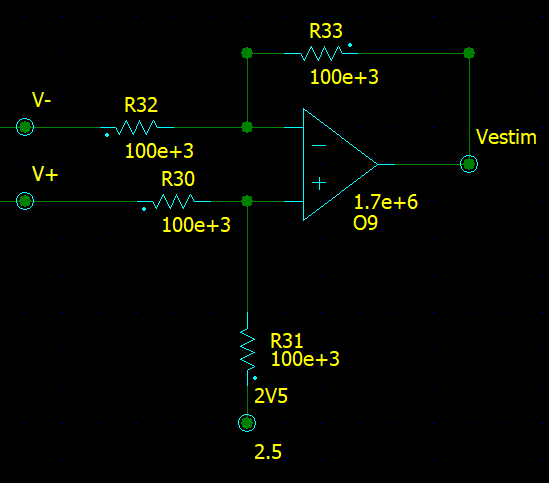
\includegraphics[scale=0.4]{Restador.png}
	\caption{Circuito restador.}
	\label{fig:img_Restador}
\end{figure}

La salida del restador está dada por:

\begin{equation} \label{eq_salida_restador}
		V_{estim}=V^+-V^-+2.5\:V
\end{equation}

Cuando $V_{deriv}$ $\mathrm{<}$ $2.5\:V$, se reemplazan los valores de $V^+$ y $V^-$ por los obtenidos en \ref{eq_V+} y \ref{eq_V-} respectivamente:

\begin{equation*} 
	\begin{aligned}
		V_{estim}&=(5\:V -\ V_{deriv})-(2.5\: V)+2.5\:V\\
		V_{estim}&=5\: V\ -\ V_{deriv}\\ 
	\end{aligned}
\end{equation*}

En este caso,  según la expresión \ref{eq_vderiv_pos}, $V_{deriv} = 2.5\:V - \abs{\Delta V_{deriv}}$. Por lo tanto:

\begin{equation*} 
	\begin{aligned}
		V_{estim}&=5\:V -(2.5\:V - \abs{\Delta V_{deriv}}) = 2.5\:V + \abs{\Delta V_{deriv}}		
	\end{aligned}
\end{equation*}

Cuando $V_{deriv}$ $\mathrm{>}$ $2.5\:V$, se reemplazan los valores de $V^+$ y $V^-$ de la ecuación \ref{eq_salida_restador} por los obtenidos en \ref{eq_V+_2} y \ref{eq_V-_2} respectivamente:

\begin{equation*} 
	\begin{aligned}
		V_{estim}&=2.5V\ -\ (5V-\ V_{deriv})+\ 2.5V\\
		V_{estim}&=V_{deriv}\\
	\end{aligned}
\end{equation*}

En este caso,  según la expresión \ref{eq_vderiv_neg}, $V_{deriv} = 2.5\:V + \abs{\Delta V_{deriv}}$. Por lo tanto:

\begin{equation*} 
	\begin{aligned}
		V_{estim}&=2.5\:V + \abs{\Delta V_{deriv}}		
	\end{aligned}
\end{equation*}

Finalmente, la tensión de salida del restador, para cualquier valor de $V_{deriv}$ se puede expresar como:

\begin{equation*} 
	\begin{aligned}
		V_{estim}&=2.5\:V + \abs{\Delta V_{deriv}}		
	\end{aligned}
\end{equation*}

\subsection{Filtrado}

En el restador se implementa un filtrado adicional a la señal de salida como se observa en la figura  \ref{fig:img_Esquema-circuital-del-restador-con-una-etapa-de-filtrado-en-159}. 

\begin{figure}[H]
	\centering
	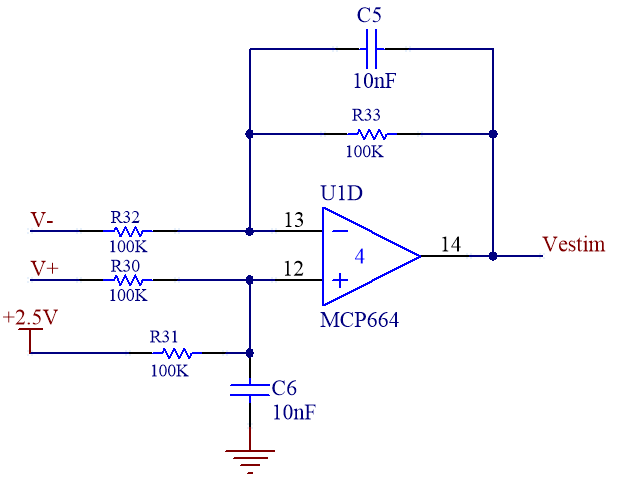
\includegraphics[scale=0.5]{Esquema-circuital-del-restador-con-una-etapa-de-filtrado-en-159.png}
	\caption{Esquema circuital del restador con una etapa de filtrado.}
	\label{fig:img_Esquema-circuital-del-restador-con-una-etapa-de-filtrado-en-159}
\end{figure}

De esta última etapa, si se considera $C_5=C_6=C\ $y $R_{33}=R_{31}=R$, se obtiene:


\begin{equation} \label{eq_Vestim_1}
	V_{estim}=\frac{1}{1+s*C*R}*(2.5\: V\ +\ |\mathit{\Delta}V_{deriv}|)
\end{equation}

\begin{equation} \label{eq_Vestim_2}
	V_{estim} \approx \frac{1}{1+s*C*R}*\ |\mathit{\Delta}V_{deriv}|\ +2.5\:V
\end{equation}

Puesto que la salida $V_{estim}$ debe ser una señal continua, es importante eliminar cualquier posible ripple. Por ello, se elige una frecuencia de corte de $1\:kr/s$ por lo que se debe cumplir que:

\begin{equation}\label{eq_filtro_restador}
	 \frac{1}{C*R}=1\:kr/s
\end{equation}

A partir de la expresión \ref{eq_filtro_restador}, se elige $C=10\: nF$ resultando en una resistencia $R=100\:k\Omega$.

\section{Simulaciones de derivador y rectificador}

A continuación se realizan simulaciones del circuito estimador conformado por los bloques derivador, rectificador y filtrado. Para ello se utilizó el software NL5 y se anexó el circuito estimador dentro del controlador de corriente. En la figura \ref{fig:img_simulacion_derivador+rectificador} se muestra el circuito utilizado para la simulación.

\begin{figure}[H]
	\centering
	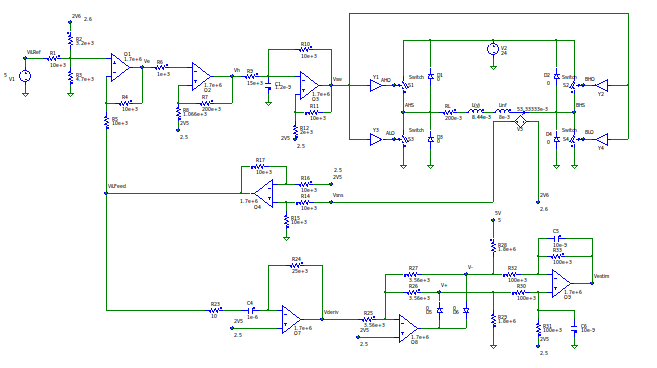
\includegraphics[scale=0.35]{simulacion_derivador+rectificador.png}
	\caption{Circuito utilizado para simulación.}
	\label{fig:img_simulacion_derivador+rectificador}
\end{figure}

\subsection{Simulación en régimen permanente} \label{sec_simulacion_estimador_basico}

Se realizó una simulación del controlador de corriente junto con el estimador, utilizando $V_{IL_{ref}}=5\:V$, que resulta en una corriente media del electroimán de $30\:A$. En la figura \ref{fig:img_simulacion_derivador+rectificador_ss} se muestran las formas de onda de la corriente del electroimán, la salida del circuito derivador, y la salida del rectificador. 

\begin{figure}[H]
	\centering
	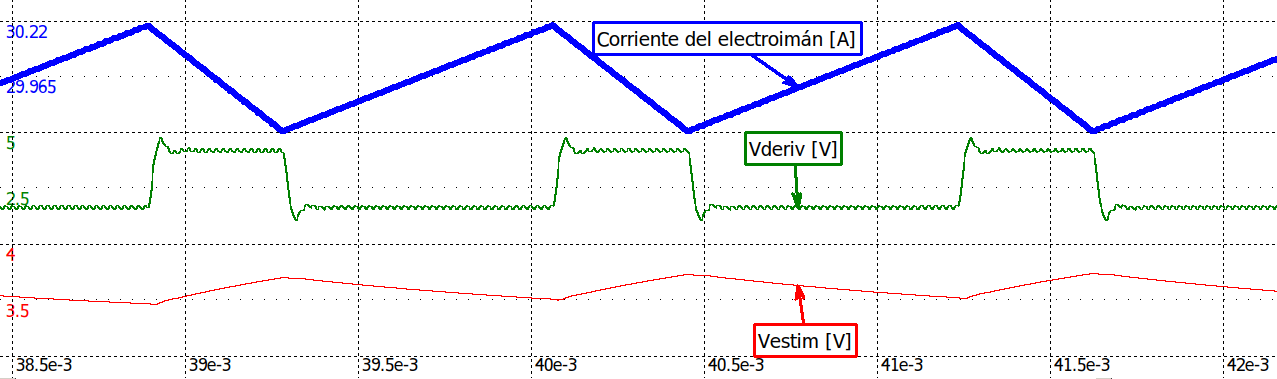
\includegraphics[scale=0.3]{simulacion_derivador+rectificador_ss.png}
	\caption{Formas de onda de corriente, salida del derivador y salida rectificada.}
	\label{fig:img_simulacion_derivador+rectificador_ss}
\end{figure}

Al observar la figura \ref{fig:img_simulacion_derivador+rectificador_ss} es posible notar dos problemas. El primero es que la forma de onda de corriente presenta pendientes de crecimiento y de decrecimiento asimétricas. Esto es provocado por el efecto de la resistencia interna del electroimán, que se hace notorio cuando se trabaja con corrientes elevadas. Esta asimetría en las pendientes provoca que la salida del derivador no sea simétrica alrededor de $V_{op}$. Por lo tanto, como luego se rectifica esta señal pulsada alrededor de $V_{op}$, la señal resultante presentará variaciones, que según mediciones realizadas con los cursores de la simulación se determinó que su amplitud es de $233\:mV$. El segundo problema es que la salida del derivador, con forma de onda pulsada, presenta un comportamiento ruidoso tanto en el nivel superior como en el inferior. Esto proviene principalmente de la conmutación auxiliar, que también es amplificada por el derivador. 

Por lo tanto, a continuación se analiza en profundidad ambos inconvenientes y se plantean soluciones a los mismos: un filtro pasa bajos en la entrada del estimador y una compensación para los efectos de la resistencia interna.

\section{Diseño del filtro pasa bajos}

Debido a que el derivador amplifica las señales de alta frecuencia se decidió agregar un filtro pasa bajos en su entrada, que permita el paso de la onda triangular de corriente pero que filtre la frecuencia de conmutación auxiliar. 

La señal que ingresa al derivador es $V_{IL_{feed}}$, que es una onda triangular de frecuencia fundamental variable entre $1\:kHz$ y $2\:kHz$. Por lo tanto se permite el paso de sus componentes frecuencia hasta la quinta armónica. De esta manera se diseña que la frecuencia de corte del filtro sea de $20\:kHz$.

Para su implementación se utiliza un filtro activo Butterworth de segundo orden, con una frecuencia de corte en $20\:kHz$. En la figura  \ref{fig:img_Filtro-para-la-entrada-del-derivador} se puede ver el circuito utilizado y en la figura \ref{fig:img_Respuesta-en-frecuencia-del-filtro-activo}, su respuesta en frecuencia.

\begin{figure}[H]
	\centering
	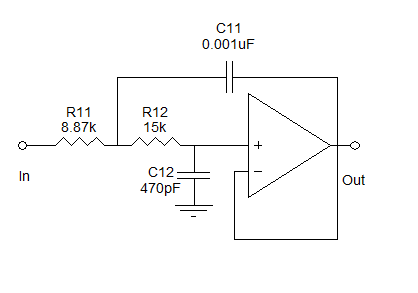
\includegraphics[scale=0.45]{Filtro-para-la-entrada-del-derivador.png}
	\caption{Filtro para la entrada del derivador.}
	\label{fig:img_Filtro-para-la-entrada-del-derivador}
\end{figure}

\begin{figure}[H]
	\centering
	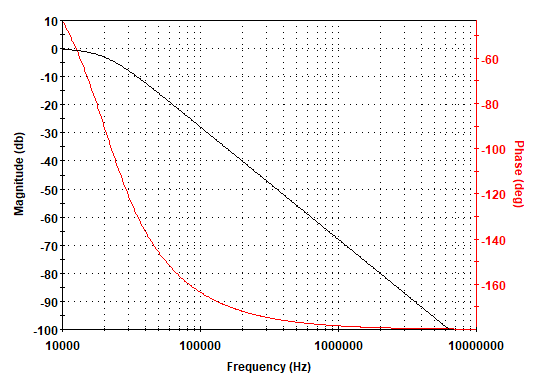
\includegraphics[scale=1]{Filtro-Activo.png}
	\caption{Respuesta en frecuencia del filtro activo.}
	\label{fig:img_Respuesta-en-frecuencia-del-filtro-activo}
\end{figure}

En la figura \ref{fig:img_simulacion_lpf_entrada} se muestra el resultado de una simulación agregando el filtro pasa bajos en la entrada. Se puede observar que, en comparación con la figura \ref{fig:img_simulacion_derivador+rectificador_ss}, la señal de salida del derivador es menos ruidosa. Esta simulación fue realizada con las mismas condiciones de corriente e inductancia que en la figura \ref{fig:img_simulacion_derivador+rectificador_ss}.

\begin{figure}[H]
	\centering
	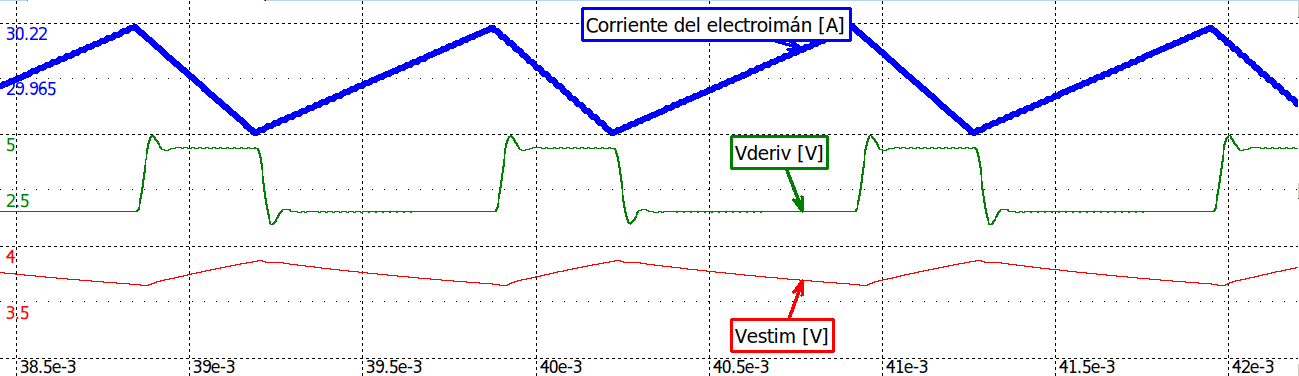
\includegraphics[scale=0.3]{simulacion_con_lpf_entrada.png}
	\caption{Simulacion del estimador con filtro pasa 	bajos en la entrada.}
	\label{fig:img_simulacion_lpf_entrada}
\end{figure}



\section{Compensación de resistencia interna}

El segundo inconveniente mencionado en la sección \ref{sec_simulacion_estimador_basico} es la diferencia entre pendientes de crecimiento y de decrecimiento causada por la resistencia interna del electroimán. A continuación se analiza cómo esta corriente provoca dicho efecto, y qué solución se propone.

Al circular corriente siempre en el mismo sentido por el electroimán, se produce una caída de tensión constante en su resistencia interna. Esto provoca que no siempre estén aplicados $\pm V_{cc}$ al electroimán sino que, durante el tiempo en que la corriente crece ($T_{ON}$) se aplican $+V_{cc}-I_L*R_L$ y durante el tiempo en que la corriente decrece ($T_{OFF}$) se aplican $-V_{cc}-I_L*R_L$. Esto genera que las pendientes sean distintas. Se puede reescribir la ecuación \ref{eq_derivada_corriente_3} para tener en cuenta el efecto mencionado, considerando que $I_L$ corresponde al valor medio de la corriente del electroimán:

\begin{equation} \label{eq_Vbus-didt-RL}
	\left|\frac{di_L}{dt}\right|=\left|\frac{\pm V_{cc}-R_L*I_L}{L(Y_g)}\right|
\end{equation}

A modo de ejemplo se plantea el caso en que circula la corriente nominal de $21\:A$ y se muestran los valores de la tensión aplicada al electroimán en el semiciclo de crecimiento y del de decrecimiento:

\begin{equation} \label{eq_Vbus-didt-RL-2}
	\abs{V_L}=\abs{\pm V_{cc}-R_L*I_L}= \abs{\pm 24\:V-4.2\:V}
\end{equation}

Para el caso en que $V_{cc}=24\:V$:

\begin{equation} \label{eq_Vbus-didt-RL-3}
	\abs{V_L}=\abs{V_{cc}-R_L*I_L}=\abs{+24\:V-4.2\:V}= 19.8\:V
\end{equation}

Para el caso en que $V_{cc}=-24\:V$:

\begin{equation} \label{eq_Vbus-didt-RL-4}
	\abs{V_L}=\abs{V_{cc}-R_L*I_L}= \abs{-24\:V-4.2\:V}= 28.2\:V
\end{equation}

Por lo tanto, sobre el electroimán se aplican dos tensiones distintas, en valor absoluto, durante la carga y descarga. Esto provoca que la rampa de corriente sea asimétrica.

Como se planteó en la sección \ref{sec_simulacion_estimador_basico}, esta diferencia de pendientes provoca que la salida del derivador no tenga una excursión simétrica al rededor del punto de operación $V_{op}=2.5\:V$. Este efecto se muestra con mayor detalle en la figura \ref{fig:img_simulacion_derivador_vmed}.

\begin{figure}[H]
	\centering
	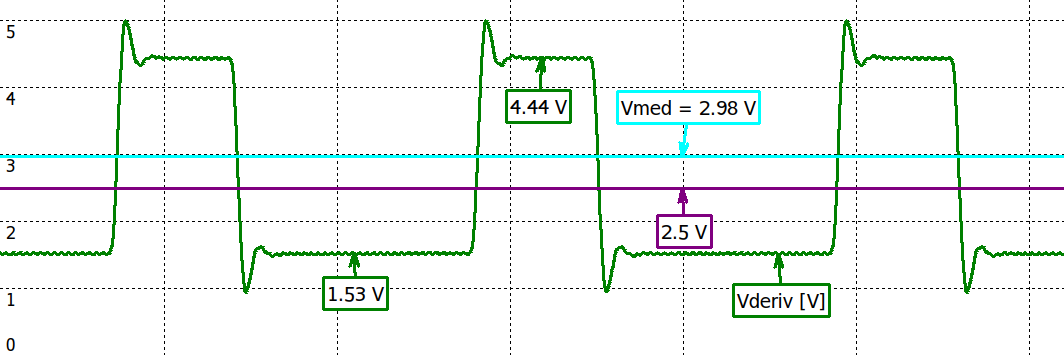
\includegraphics[scale=0.3]{simulacion_derivador_vmed.png}
	\caption{Salida del derivador mostrando valor medio y Vmed.}
	\label{fig:img_simulacion_derivador_vmed}
\end{figure}

En la figura \ref{fig:img_simulacion_sin_compensacion_IR} se muestra la señal $V_{estim}$ sin la etapa de filtrado del restador, para que se vea mas claro el efecto provocado al rectificar la salida del derivador. 

%Debido a que luego se utilizará un rectificador de onda completa, se desea que la rectificación de cada una de estas pendientes resulte en el mismo valor. En la figura \ref{fig:img_Forma-de-onda-luego-de-rectificar-sin-compensación-IR} se muestra el efecto luego de la rectificación sin realizar ninguna compensación.

\begin{figure}[H]
	\centering
	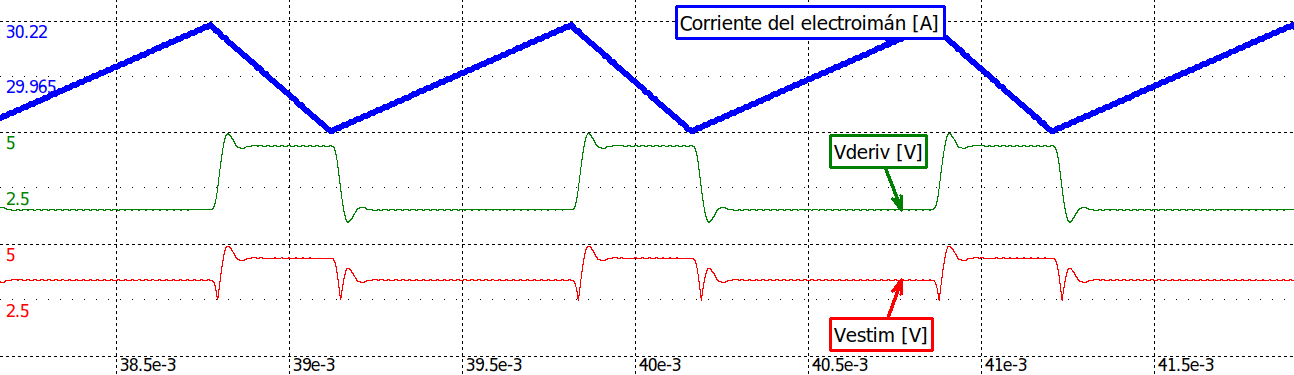
\includegraphics[scale=0.3]{simulacion_sin_compensacion_IR.png}
	\caption{Forma de onda luego de rectificar sin compensación de resistencia interna.}
	\label{fig:img_simulacion_sin_compensacion_IR}
\end{figure}

La solución a este problema es hacer que el valor $V_{med}$ mostrado en la figura \ref{fig:img_simulacion_derivador_vmed} coincida con $V_{op}$. Para lograrlo se debe modificar el punto de operación de la salida del derivador, de manera de compensar el término $\frac{R_L*I_L}{L(Y_g)}$ que se agrega.

Para modificar el punto de operación se debe cambiar la tensión en la entrada no inversora del circuito derivador ($V_{bias}$) como se muestra en la figura \ref{fig:img_Esquema-circuital-del-derivador}. 

\begin{figure}[H]
	\centering
	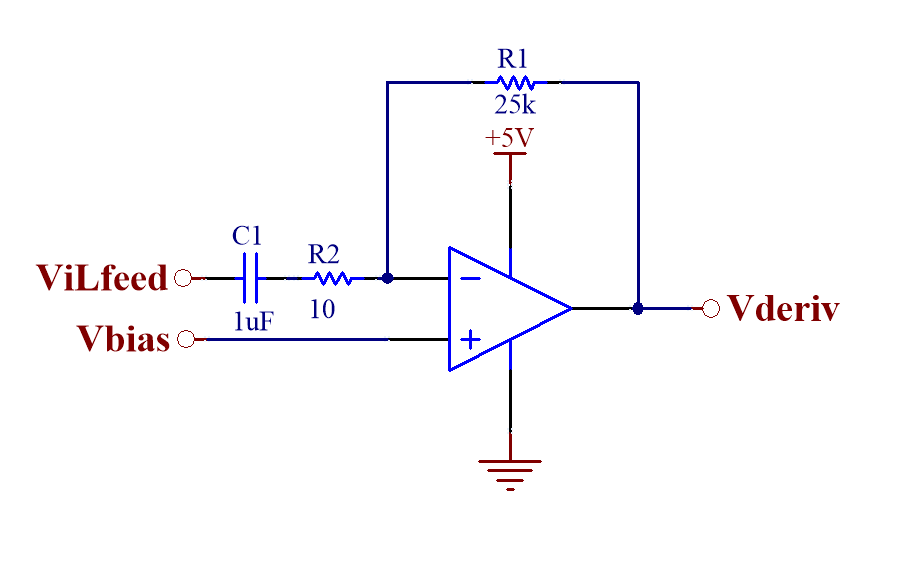
\includegraphics[scale=0.5]{Esquema-circuital-del-derivador.png}
	\caption{Esquema circuital del derivador con $V_{bias}$.}
	\label{fig:img_Esquema-circuital-del-derivador}
\end{figure}

La pendiente de bajada de la onda triangular, en módulo, es mayor que la de subida. Por lo tanto, al derivarla (con la inversión de signo), queda por encima del punto de operación, y la pendiente de subida, por debajo. Por ello, se debe compensar el punto de operación para que la forma de onda sea simétrica alrededor de $2.5\:V$. 

Para la pendiente de bajada, la salida del derivador es:

\begin{equation} \label{eq_Vyf-Vbias}
	V_{deriv_{sup}} =\ V_{bias}+H_0\ *\ \tau *\frac{\abs{V_{cc}}\ +\ I_L*R_L}{L(Y_g)}\ 
\end{equation}

Para la pendiente de subida:

\begin{equation} \label{eq_Vyf-Vbias2}
	V_{deriv_{inf}} =\ V_{bias}\ -\ H_0\ *\ \tau *\frac{\abs{V_{cc}} -\ I_L*R_L}{L(Y_g)}
\end{equation}

Se desea que se cumpla:

\begin{equation} \label{eq_Vyf_Vbias3}
	V_{deriv_{sup}} -2.5\:V=\ 2.5\:V\ - V_{deriv_{inf}}
\end{equation}

Si se despeja $V_{bias}$ se llega a:

\begin{equation} \label{eq_Vyf-Vbias4}
	V_{bias}\ =2.5 \:V -\ H_0\ *I_L*\ \tau *\frac{\ R_L}{L(Y_g)}
\end{equation}

Para generar la tensión $V_{bias}$ se debe implementar un circuito que mida el valor medio de la corriente del electroimán y entregue en su salida la tensión que indica la expresión \ref{eq_Vyf-Vbias4}. Como no se tiene acceso directo a la corriente del electroimán, sino que se tiene la tensión de realimentación de corriente $V_{IL_{feed}}=H_0*I_L+0.1\:V$, se utiliza esta tensión como entrada. Se propone el circuito de la figura \ref{fig:img_Generación_de_Vbias}.

\begin{figure}[H]
	\centering
	\includegraphics[scale=0.6]{Generación-de-Vbias.png}
	\caption{Generación de $V_{bias}$.}
	\label{fig:img_Generación_de_Vbias}
\end{figure}

El capacitor $C_1$ cumple la función de obtener el valor medio de la señal de entrada, que tiene forma triangular con frecuencia mínima de $1\:kHz$. Se elige su valor para que, junto con la resistencia $R_4$, filtre la frecuencia fundamental de la onda triangular. Por lo tanto, se ubica la frecuencia de corte una década por debajo y se impone la siguiente condición de diseño:

\begin{equation} \label{eq_capacitor_IR}
	\frac{1}{2*\pi*C_1*R_4}=100\:Hz
\end{equation}



A partir del circuito de la figura \ref{fig:img_Generación_de_Vbias} se obtiene:

\begin{equation} \label{eq_Vyf-Vbias3}
	V_{bias} =V_{op}(1+\frac{ R_4}{R_3(1+sC_1R_4)})(\frac{R_1}{R_1+R_2})-\frac{R_4(V_{IL_{feed}})}{R_3(1+s C_1R_4)}
\end{equation}

Como se mencionó previamente, el capacitor $C_1$ junto con $R_4$ se encargan de filtrar las señales de entrada y obtener a la salida del circuito su valor medio. Por lo tanto, para simplificar el análisis, se plantea la siguiente ecuación:

\begin{equation} 
	V_{bias} =V_{op}(1+\frac{ R_4}{R_3})(\frac{R_1}{R_1+R_2})-\frac{R_4(I_L*H_0+0.1\:V)}{R_3}
\end{equation}


Para poder llegar a la expresión de la ecuación \ref{eq_Vyf-Vbias4} se debe cumplir que:

\begin{enumerate}
	\item  $-\frac{R_4}{R_3}=- \tau *\frac{R_L}{L}= -0.304$  
	
	\item  $-\frac{R_4}{R_3}(0.1V)+V_{op}(1+\frac{ R_4}{R_3})(\frac{R_1}{R_1+R_2}) = 2.5V$     
\end{enumerate}

Se sabe que $H_0 = 53.3\:\frac{mV}{A},\; R_L = 0.2\:\Omega$ y $\tau=C_1*R_1=25 \:ms$. Se utiliza la inductancia $L(4\:mm) = 16.44\:mHy$.

Por lo tanto, al resolver la condición 1) se elige $R_4 = 304\: \Omega$ y se obtiene $R_3=1\:k\Omega$. Luego, al resolver la condición 2) con $V_{op}=2.5\:V$ se elige $R_1=1\:k\Omega$ y se obtiene $R_{2}=291.8\:\Omega$. Finalmente, siguiendo la condición \ref{eq_capacitor_IR}, se determina $C_1=5.14\mu F$.

Se simuló nuevamente el circuito estimador con el agregado de la compensación de resistencia interna. En la figura \ref{fig:img_Formas_de_onda_obtenidas_en_la_simulación} se muestra cómo mejoró la forma de onda a la salida del rectificador.

\begin{figure}[H]
	\centering
	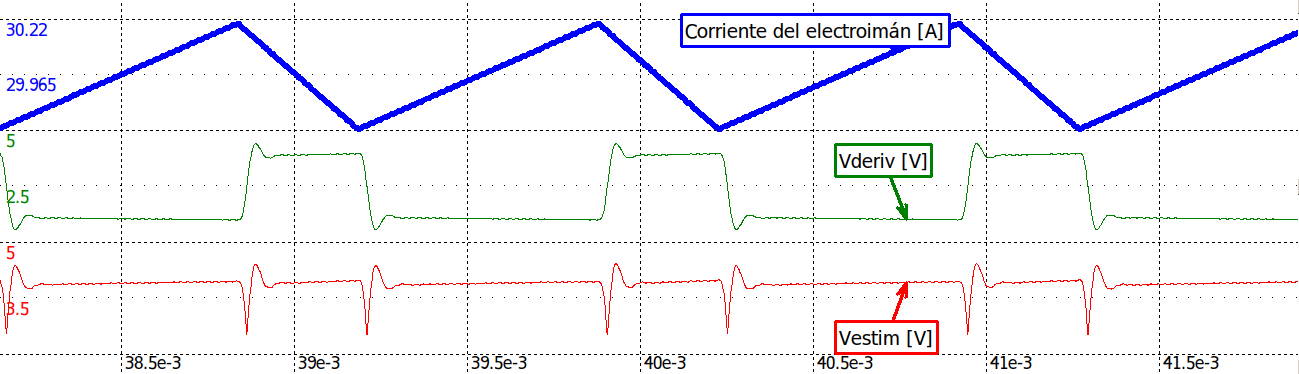
\includegraphics[scale=0.3]{simulacion_compensacion_IR.png}
	\caption{Formas de onda obtenidas en la simulación.}
	\label{fig:img_Formas_de_onda_obtenidas_en_la_simulación}
\end{figure}


\section{Simulación del estimador completo}

Finalmente el circuito estimador completo y la simulación se muestran en las figuras \ref{fig:img_circuito_final_del_estimador} y \ref{fig:img_simulacion_completo} respectivamente.

\begin{figure}[H]
\centering
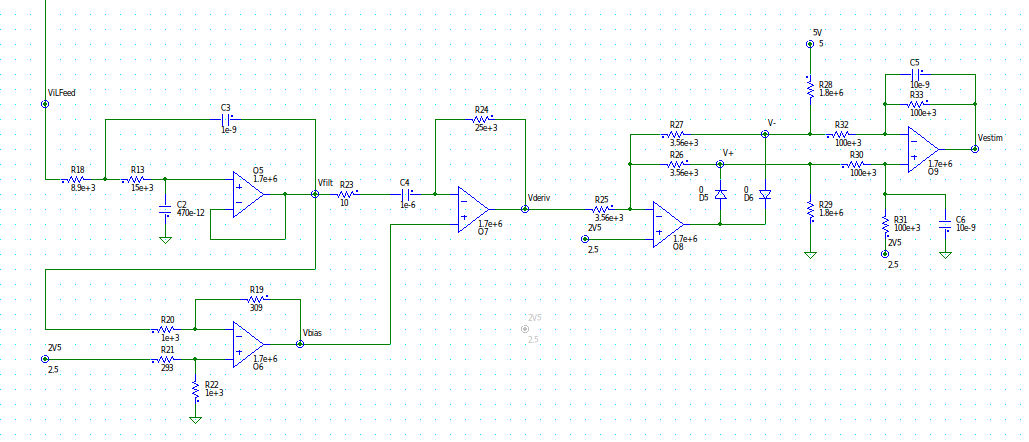
\includegraphics[scale=0.3]{circuito_completo.png}
\caption{Circuito final del estimador.}
\label{fig:img_circuito_final_del_estimador}
\end{figure}

\begin{figure}[H]
	\centering
	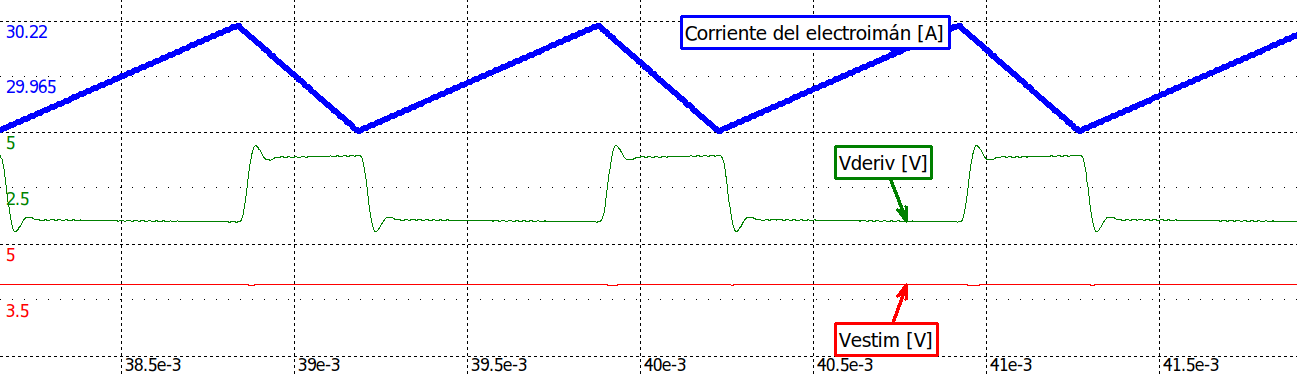
\includegraphics[scale=0.3]{simulacion_completo.png}
	\caption{Simulación del circuito estimador completo.}
	\label{fig:img_simulacion_completo}
\end{figure}

Se puede observar que la salida del estimador $V_{estim}$ es una señal aproximadamente continua. Mediante la utilización de los cursores se midió una variación de $97\:mV$ en torno al valor medio, resultando en una mejora con respecto a la simulación realizada en la figura \ref{fig:img_simulacion_derivador+rectificador_ss}, en la que las variaciones de amplitud eran de $233\:mV$.

Se realizó la tabla \ref{tab_Resultados_de_simulación_del_estimador} que muestra el valor resultante y los calculados teóricamente (\ref{tab_Vyf_vs_y}) de $V_{estim}$ en la simulación para distintos casos de distancia de entrehierro. En ella también se agrega una columna con los valores teóricos calculados en \ref{tab_derivada_linealizada} para realizar una comparación.
\colorbox{red}{Agregar valores teoricos y medidos y hacer análisis de la diferencia entre ellos, y calcular la pendiente...}

\begin{table}[H]
	\begin{center}
		\begin{tabular}{| c | c | c | c |}
			\hline
			$Y_g\:[mm]$ & $L(Y_g)\:[mHy]$ & $V_{estim_{teorico}}\:[V]$ & $V_{estim_{simulado}}\:[V]$ \\ \hline 
			2 & 22.64 & 3.92 &3.58 \\ \hline 
			3 & 18.8 & 4.18 &3.82 \\ \hline 
			4 & 16.44 & 4.44 &3.93 \\ \hline 
			5 & 14.9 & 4.7 &4.06 \\ \hline 
		\end{tabular}
		\caption{Resultados de simulación del estimador.}
		\label{tab_Resultados_de_simulación_del_estimador}
	\end{center}
\end{table}

En la tabla \ref{tab_Resultados_de_simulación_del_estimador} se observa que los valores obtenidos en simulación son menores que los calculados teóricamente. Esta diferencia se debe a que para los cálculos teóricos se utilizó $V_{cc}=24$, pero por la conmutación auxiliar es menos..... sigo maañana



\section{Transferencia final del estimador de posición}

El comportamiento del circuito estimador no es lineal.  Por lo tanto, para poder modelar una función transferencia, se deben tomar ciertas consideraciones. La parte del derivador es lineal, por lo que se puede modelar su transferencia como:
\begin{equation}\label{eq_v-estim}
	V_{deriv}=-0.025*\frac{dV_{IL_{feed}}}{dt} 
\end{equation}

A partir de la expresión \ref{eq_v-estim} se puede determinar que, además de realizarse la derivada, se introduce una inversión de signo. De esta forma, una pendiente positiva a la entrada resulta en valores menores a $2.5\:V$ a la salida, mientras que una pendiente negativa produce una tensión mayor a $2.5\:V$.

Luego, el bloque rectificador y restador se encarga de calcular el valor absoluto de esta señal (en torno a los $2.5\:V$). Al considerar que la pendiente aumenta a medida que lo hace la distancia de separación, se puede concluir que el bloque estimador no produce inversión de signo. Por lo tanto, se debe considerar solamente la ganancia del derivador y el polo que introduce la etapa de restador. Por lo tanto la salida del estimador en función de la salida del derivador queda:

\begin{equation} \label{eq_vestim_dvil}
	V_{estim}=0.025*\abs{\frac{dV_{IL_{feed}}}{dt}}*\frac{1}{1+\frac{s}{1\:kr/s}} 
\end{equation}


Finalmente, para poder obtener una estimación de la posición, se utiliza la expresión linealizada \ref{eq_di-dt_lineal} que relaciona la derivada de la corriente con el entrehierro:

\begin{equation} \label{eq_dil_yg}
	\abs{\frac{dI_{L}}{dt}} = 194690 * Y_{g}
\end{equation}


Al considerar la ganancia que tiene el sensor de efecto Hall sobre la corriente:

\begin{equation} \label{eq_dil_dvil}
	\abs{\frac{dV_{IL_{feed}}}{dt}}= H_0*\frac{dI_{L}}{dt} 
\end{equation}

Por lo tanto al reemplazar la expresión \ref{eq_dil_yg} en \ref{eq_dil_dvil} se obtiene \ref{eq_dvil_yg_2}.

\begin{equation} \label{eq_dvil_yg_2}
	\abs{\frac{dV_{IL_{feed}}}{dt}} = H_0*194690*Y_{g}
\end{equation}

Utilizando el resultado de \ref{eq_dvil_yg_2} en \ref{eq_vestim_dvil} se llega a:

\begin{equation}
	V_{estim}=0.025*194690*0.0533 * \frac{Y_{g}}{1 + \frac{s}{1\:kr/s}}=259.6*\frac{Y_{g}}{1 + \frac{s}{1\:kr/s}}	
\end{equation}

Finalmente, al considerar la etapa de filtrado de la entrada, que tiene dos polos en $2\pi *10\:{kHz} \simeq 60 \:{kr/s}$ se obtiene:

\begin{equation} \label{eq_TLC_deriv_7}
	H_{estim}=\frac{V_{estim}}{Y_{g}[m]}=\frac{259.6}{(1+\frac{s}{1\:k})*{(1+\frac{s}{60\: k})}^2}
\end{equation}

